\chapter{Evaluation}
\label{ch:evaluation}

%Describe the approaches you have used to evaluate that the solution you have designed in \Cref{ch:design} and executed in \Cref{ch:implementation} actually solves the problem identified in \Cref{ch:introduction}.

%While you can discuss unit testing etc. you have carried here a little bit, that is the minimum. You should present data here and discuss that. This might include \emph{e.g.} performance data you have obtained from benchmarks, survey results, or application telemetry / analytics. Tables and graphs displaying this data are good.

关于测试连通性以及圆中是否有4个以上格点,分别调用$solver._domain.test_connection$和$solver._domain._cycle.Isvalid()$即可.

在这里针对各种情况的计算结果.

如果你想要自己完成计算,请按以下步骤操作:
\begin{itemize}
    \item 在FunctionExtension.h中公开继承Function类,实现其中的括号运算符.
    \item 仿照input中的示例填写json文件
    \item 在main函数中调用JsonRead函数,会执行计算并将计算结果输出到output中,四列数据分别代表该点的列数,行数,计算值,绝对误差
    \item 在plot文件夹的python文件中实现画图(画图函数已实现,只需将文件的名字作为参数,会自动检索output中同名文件,输出结果在image中)
\end{itemize}

\section{计算结果}

\subsection{计算实例命名}

为方便查找想要看的计算结果,这里给出相应的命名规范
\begin{itemize}
    \item 开头为格点数减一的值,如$n8$,$n16$,$n32$,$n64$
    \item 其次为第几个函数,如$f1$,$f2$
    \item 再然后为非圆上的边界条件类型$d$表示$Dirichlet$条件,$m$表示$Mixed$条件(由于neumann条件在常数意义下有无穷解,需要设定一个dirichlet条件的点,所以也视为mixed)
    \item 若接着一个$c$,表示定义域扣去了一个圆盘
    \item 若有$c$,则会跟随一个表示圆上边界条件类型的符号(圆和非圆边界有一个有Dirichlet条件即可,为方便,测试时还是命名为m和d)
\end{itemize}

\subsection{q-norm随网格细分变化}

结合随$n$变化的图像,可知对算例总体而言,随n变大,误差变小.
从随$h$变化的图像,关于$h$成线性关系.
以下第一张图为随n变化图像,第二张图为随h变化图像.

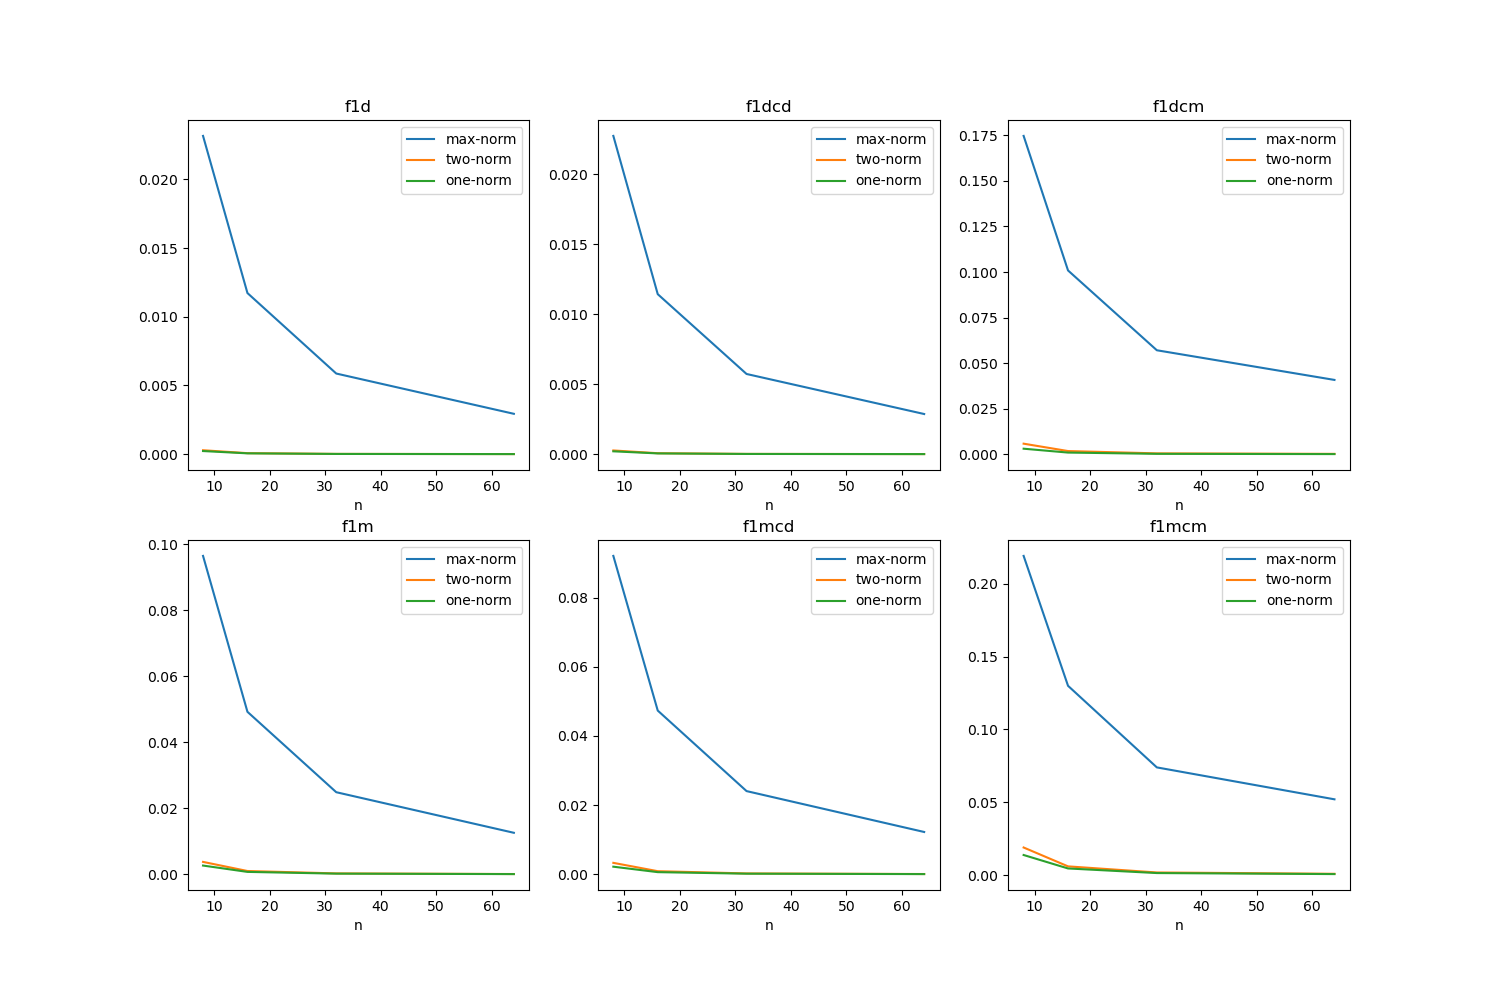
\includegraphics[scale=0.4]{../../image/nnorm.png}

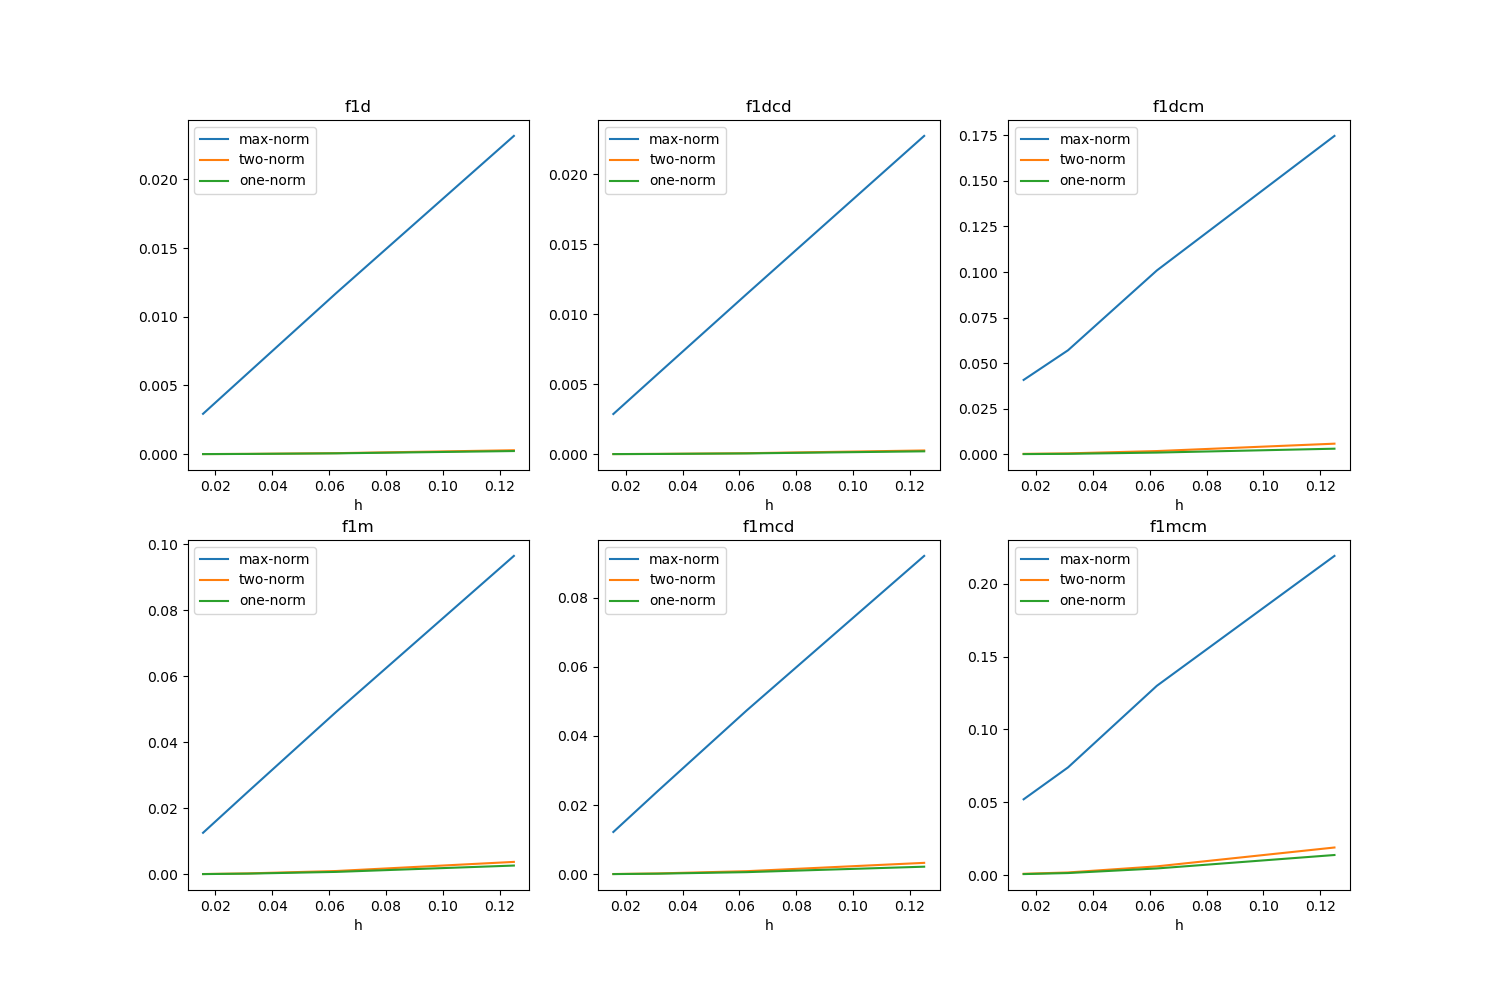
\includegraphics[scale=0.4]{../../image/hnorm.png}

\subsection*{n8f1d}
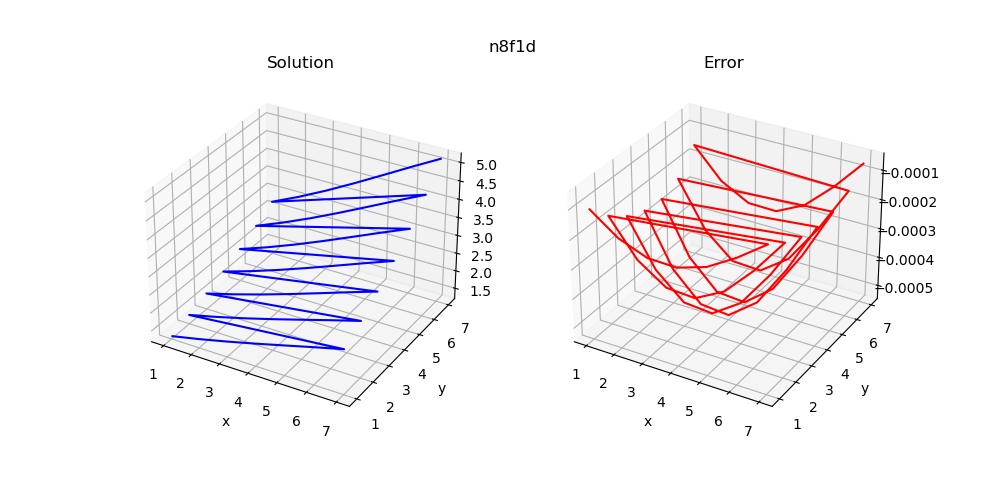
\includegraphics[scale=0.6]{../../image/n8f1d.png}
\subsection*{n8f1dcd}
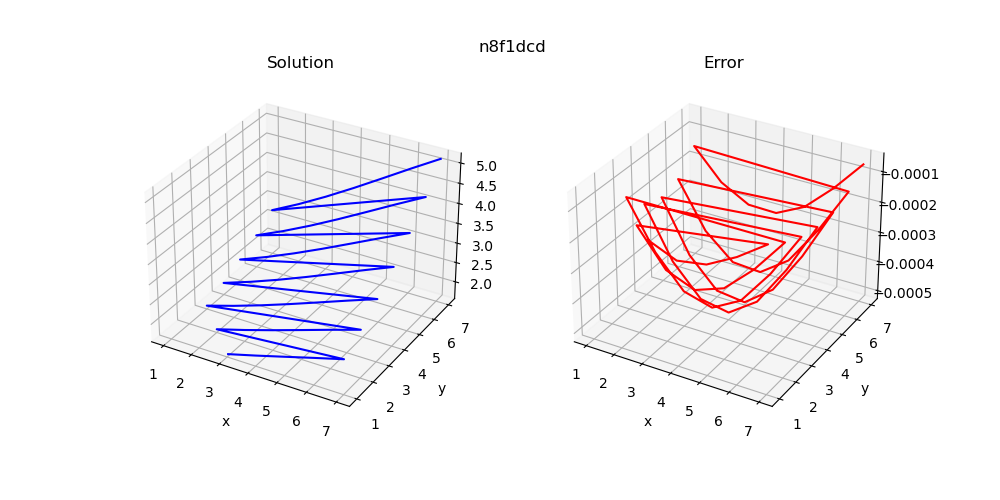
\includegraphics[scale=0.6]{../../image/n8f1dcd.png}
\subsection*{n8f1dcm}
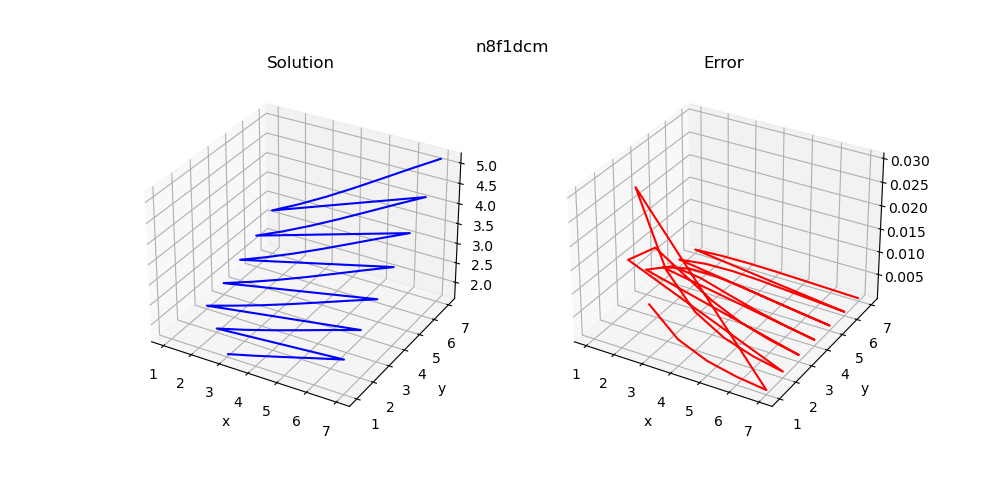
\includegraphics[scale=0.6]{../../image/n8f1dcm.png}
\subsection*{n8f1m}
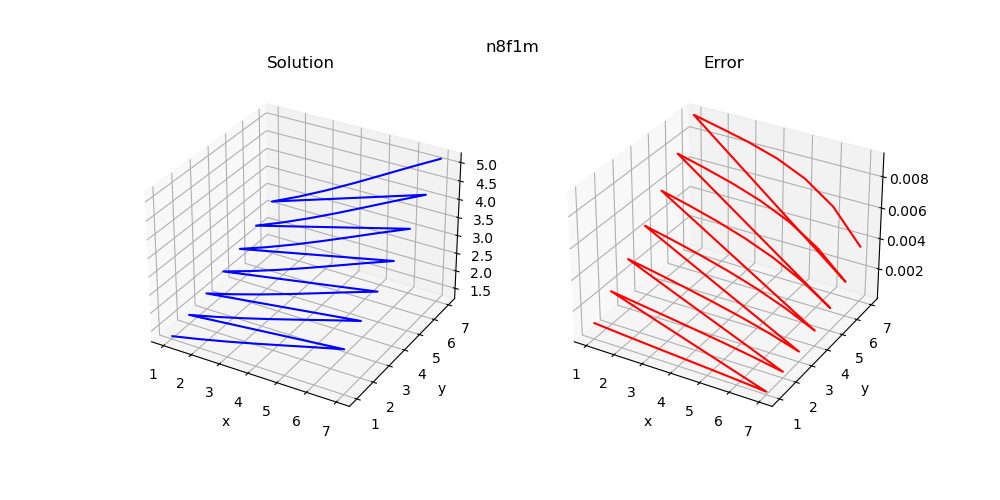
\includegraphics[scale=0.6]{../../image/n8f1m.png}
\subsection*{n8f1mcd}
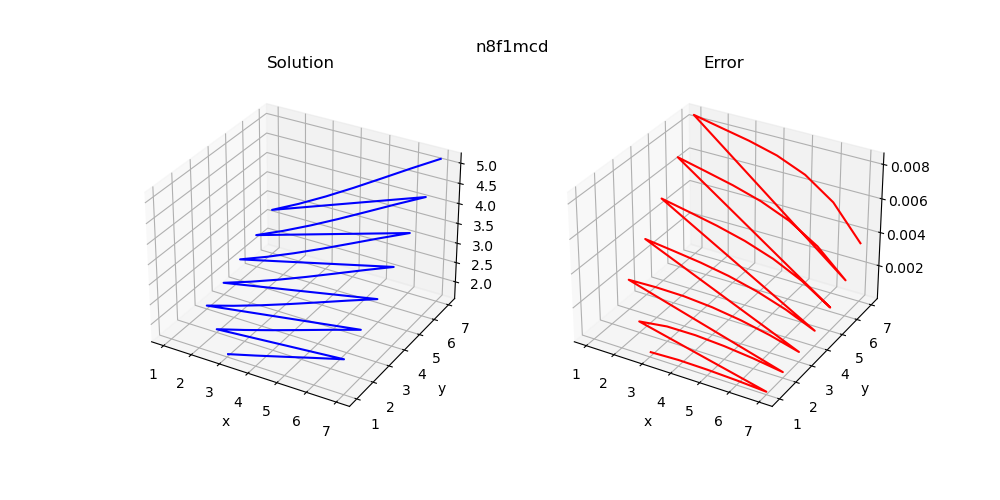
\includegraphics[scale=0.6]{../../image/n8f1mcd.png}
\subsection*{n8f1mcm}
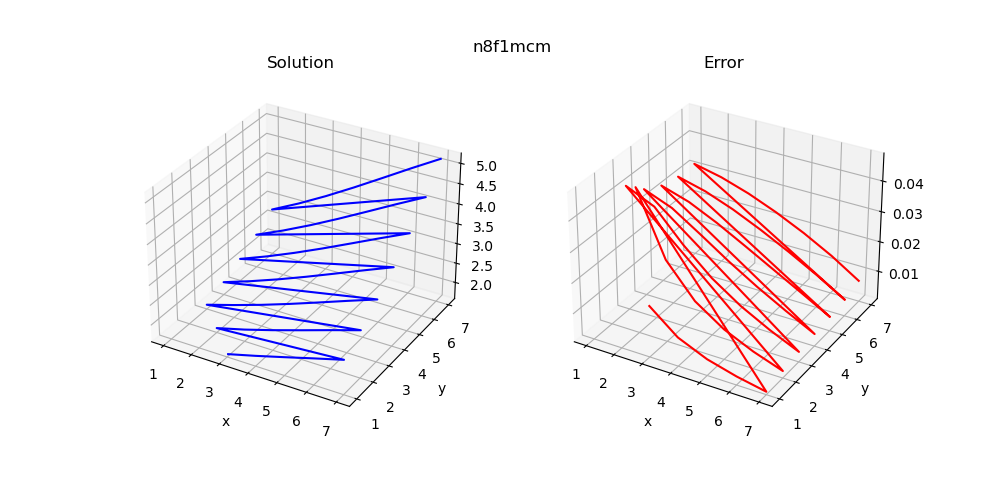
\includegraphics[scale=0.6]{../../image/n8f1mcm.png}
\subsection*{n16f1d}
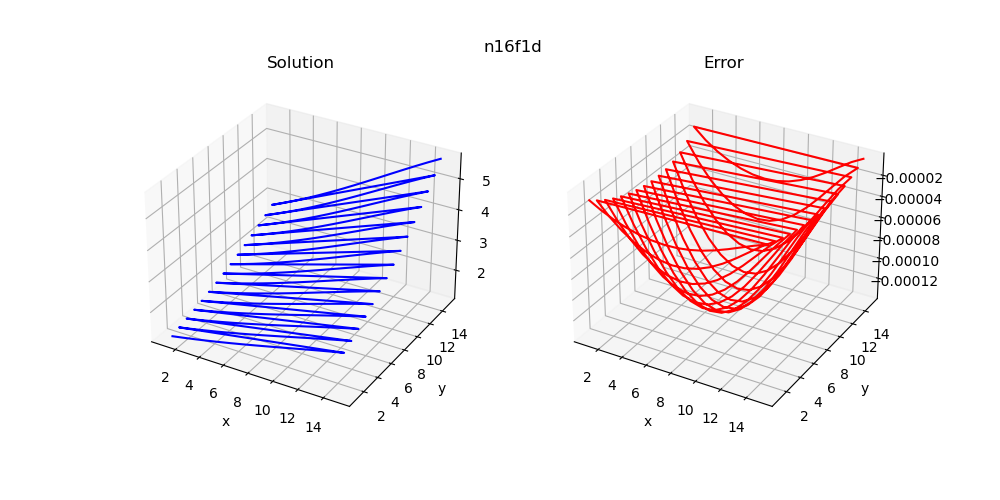
\includegraphics[scale=0.6]{../../image/n16f1d.png}
\subsection*{n16f1dcd}
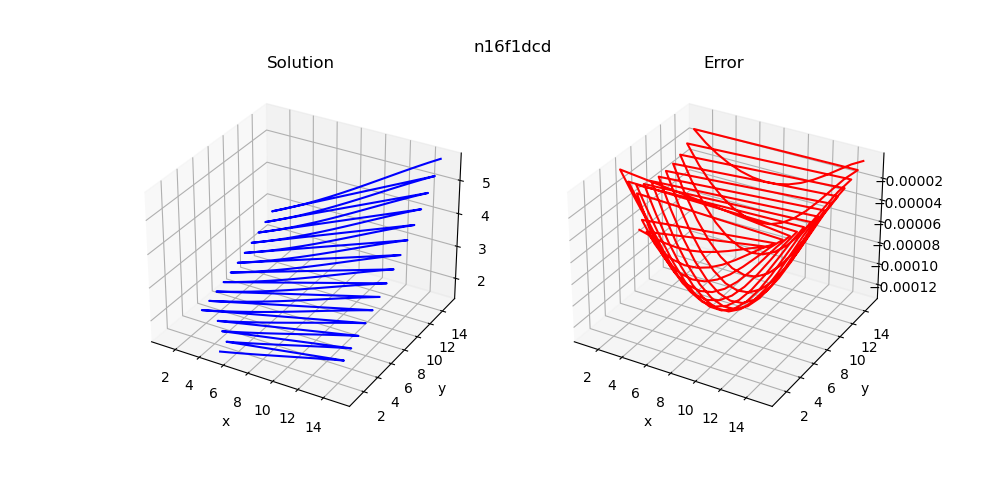
\includegraphics[scale=0.6]{../../image/n16f1dcd.png}
\subsection*{n16f1dcm}
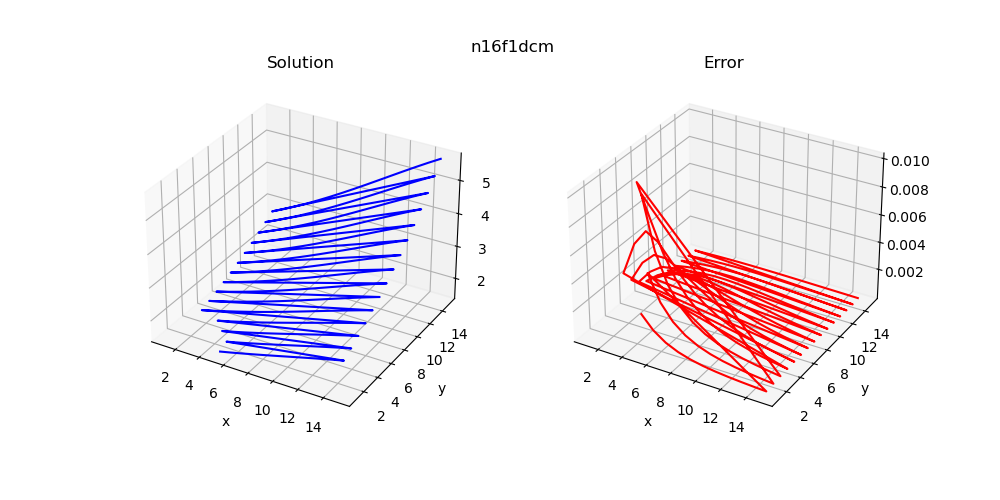
\includegraphics[scale=0.6]{../../image/n16f1dcm.png}
\subsection*{n16f1m}
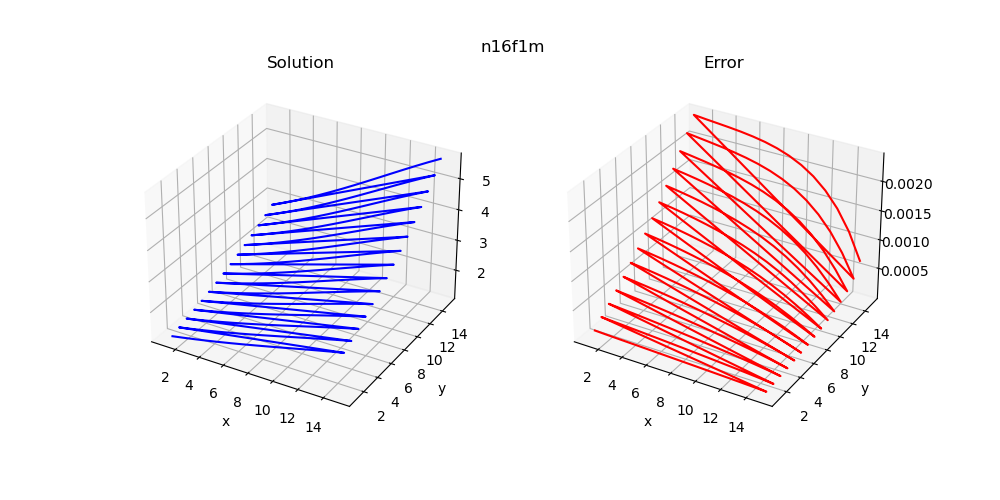
\includegraphics[scale=0.6]{../../image/n16f1m.png}
\subsection*{n16f1mcd}
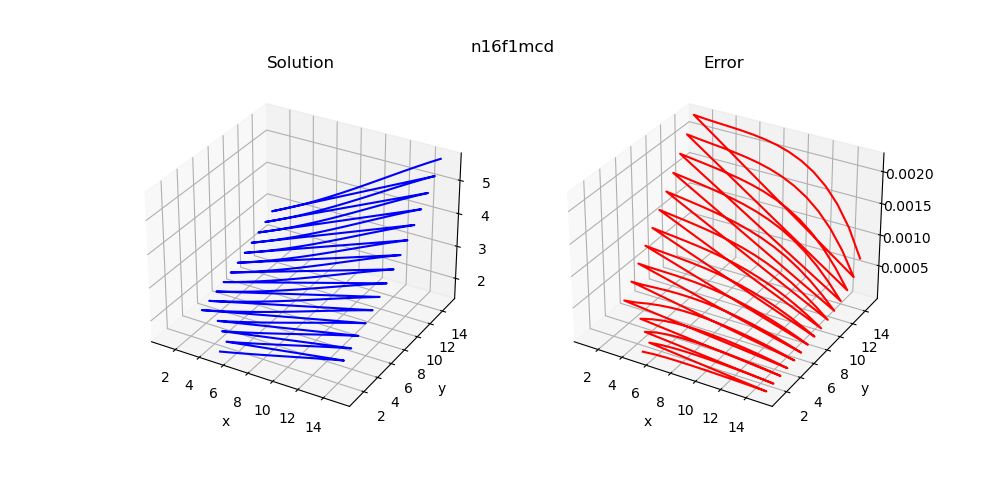
\includegraphics[scale=0.6]{../../image/n16f1mcd.png}
\subsection*{n16f1mcm}
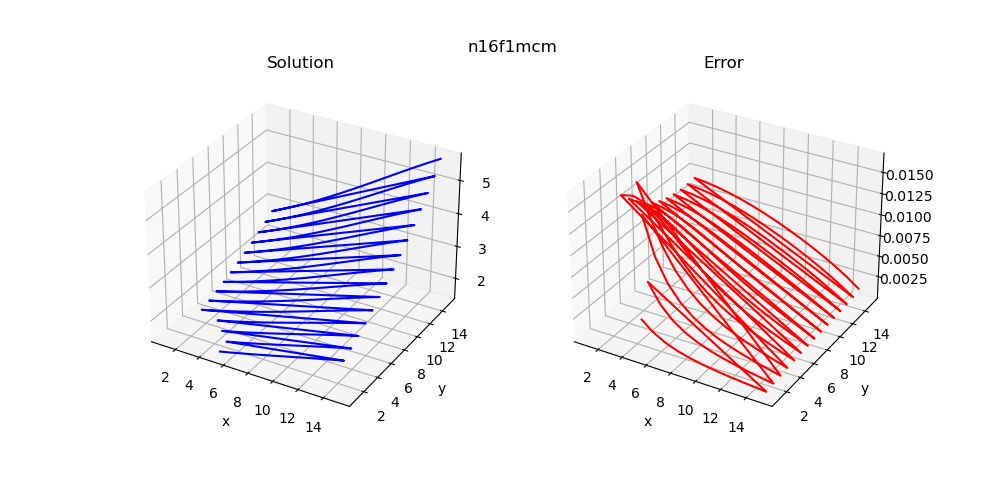
\includegraphics[scale=0.6]{../../image/n16f1mcm.png}
\subsection*{n32f1d}
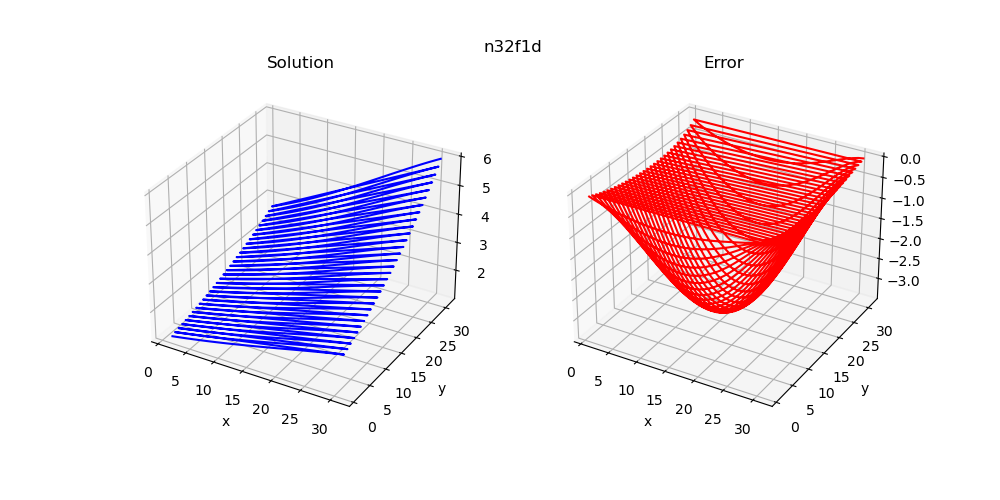
\includegraphics[scale=0.6]{../../image/n32f1d.png}
\subsection*{n32f1dcd}
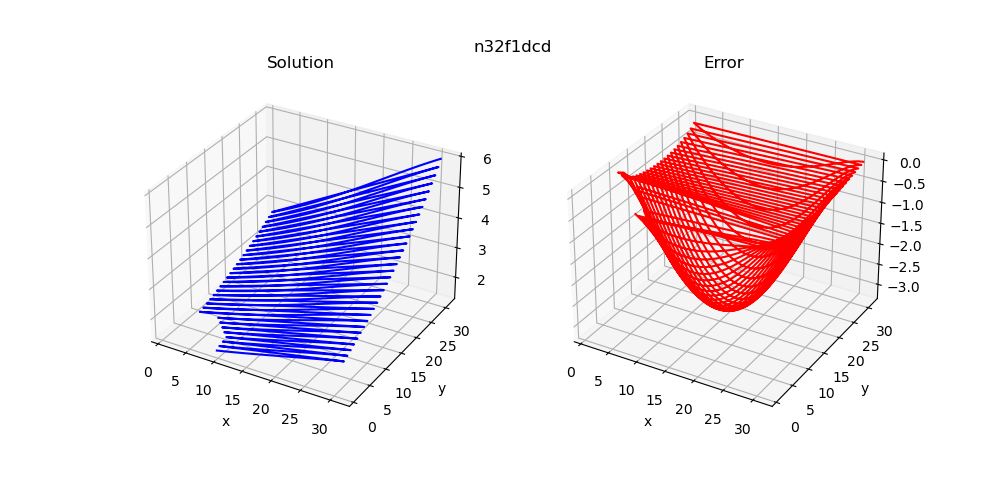
\includegraphics[scale=0.6]{../../image/n32f1dcd.png}
\subsection*{n32f1dcm}
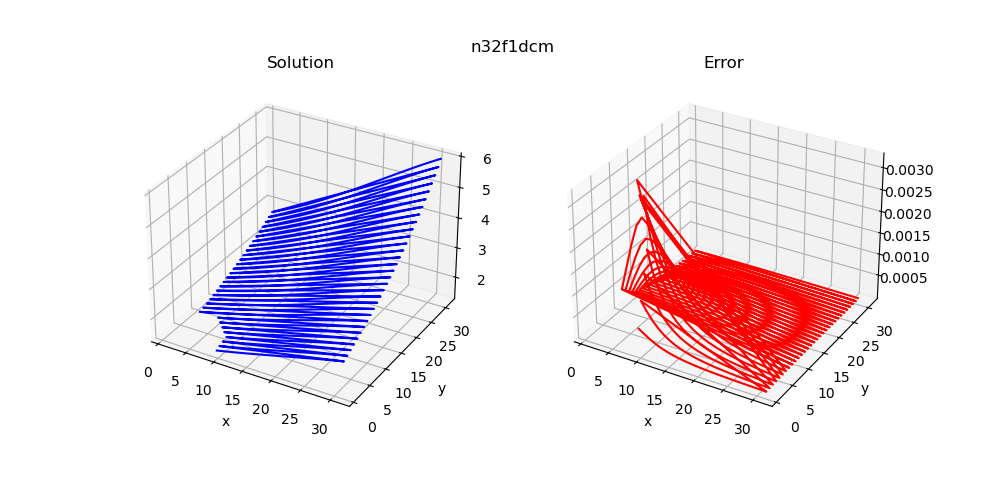
\includegraphics[scale=0.6]{../../image/n32f1dcm.png}
\subsection*{n32f1m}
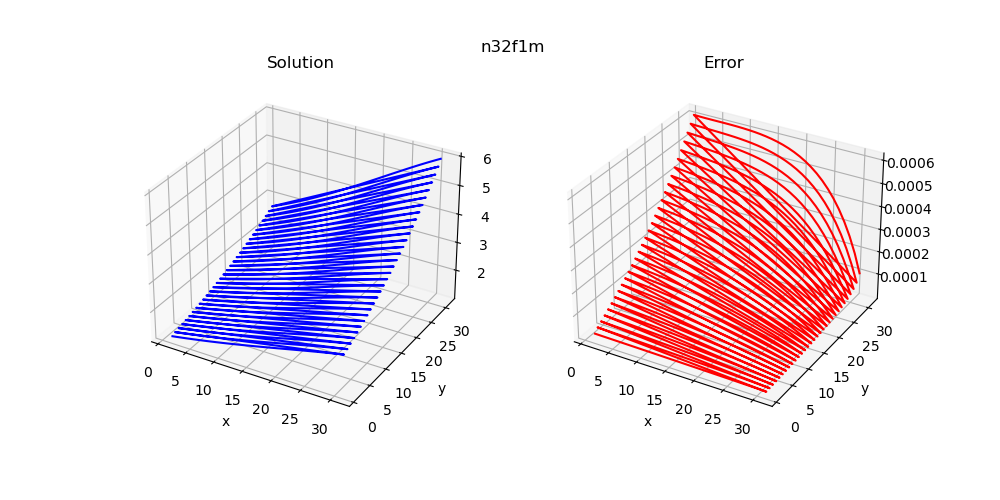
\includegraphics[scale=0.6]{../../image/n32f1m.png}
\subsection*{n32f1mcd}
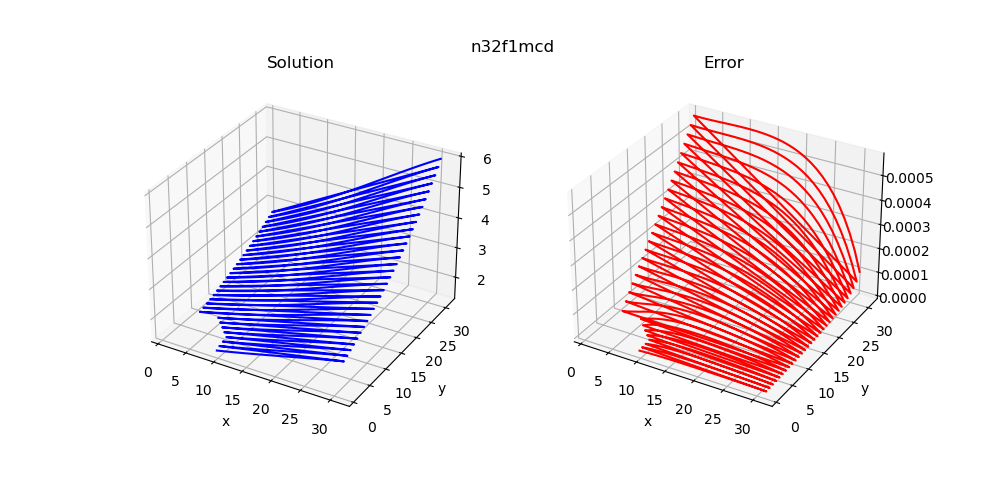
\includegraphics[scale=0.6]{../../image/n32f1mcd.png}
\subsection*{n32f1mcm}
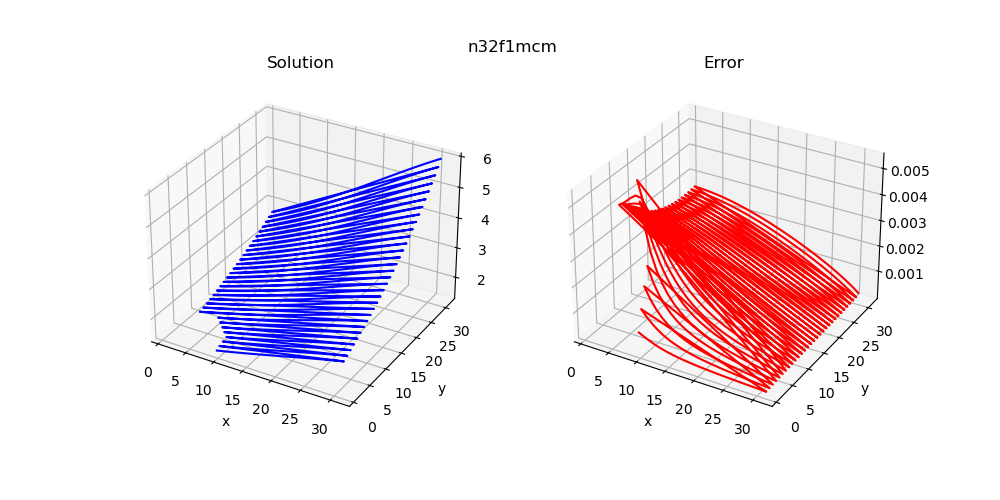
\includegraphics[scale=0.6]{../../image/n32f1mcm.png}
\subsection*{n64f1d}
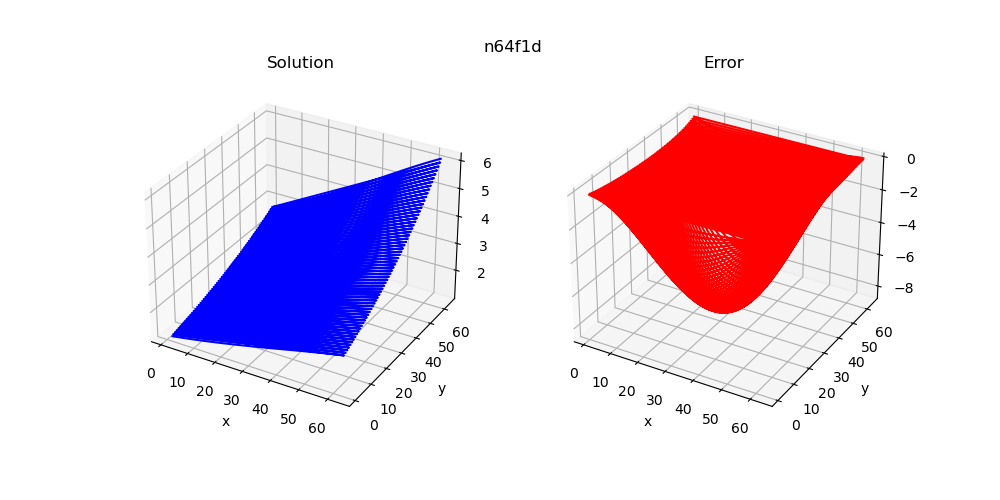
\includegraphics[scale=0.6]{../../image/n64f1d.png}
\subsection*{n64f1dcd}
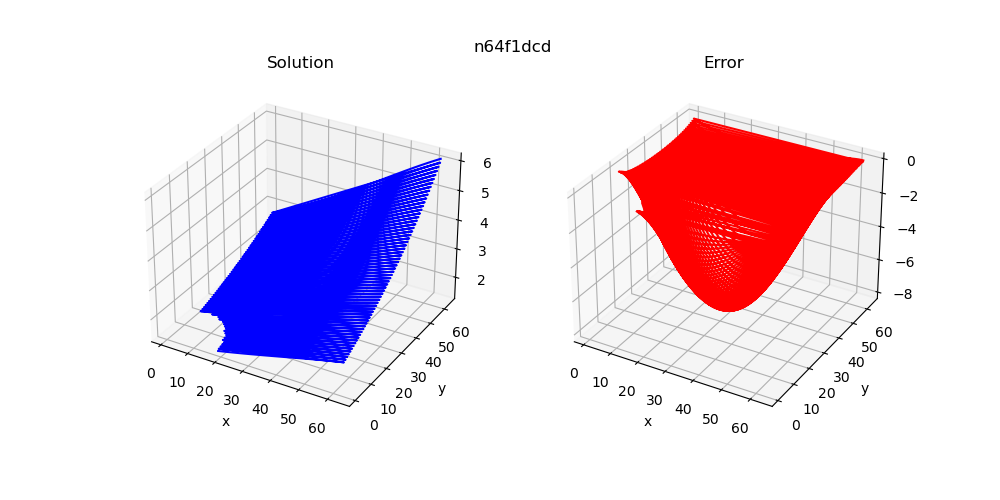
\includegraphics[scale=0.6]{../../image/n64f1dcd.png}
\subsection*{n64f1dcm}
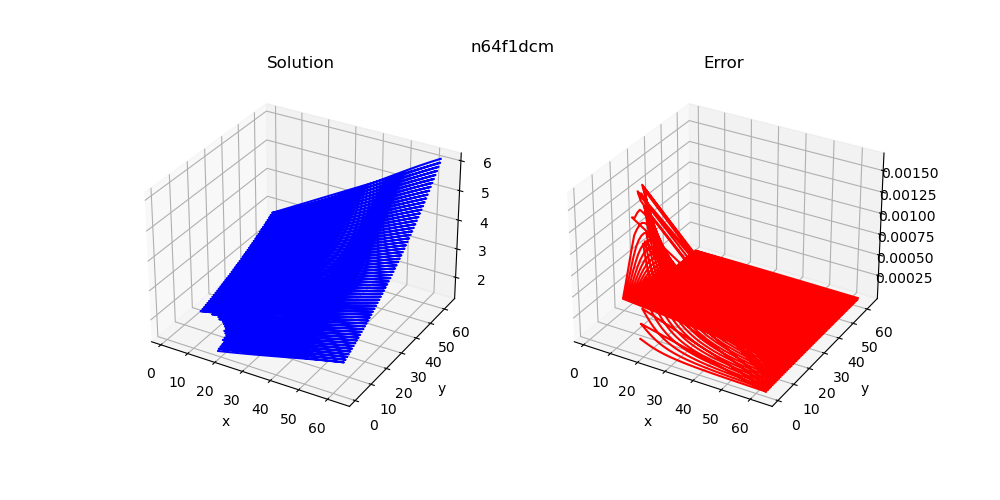
\includegraphics[scale=0.6]{../../image/n64f1dcm.png}
\subsection*{n64f1m}
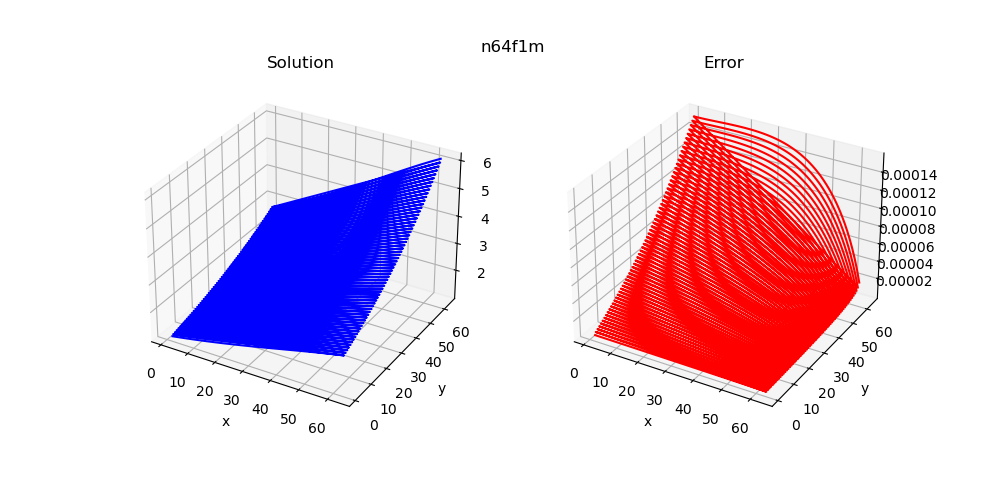
\includegraphics[scale=0.6]{../../image/n64f1m.png}
\subsection*{n64f1mcd}
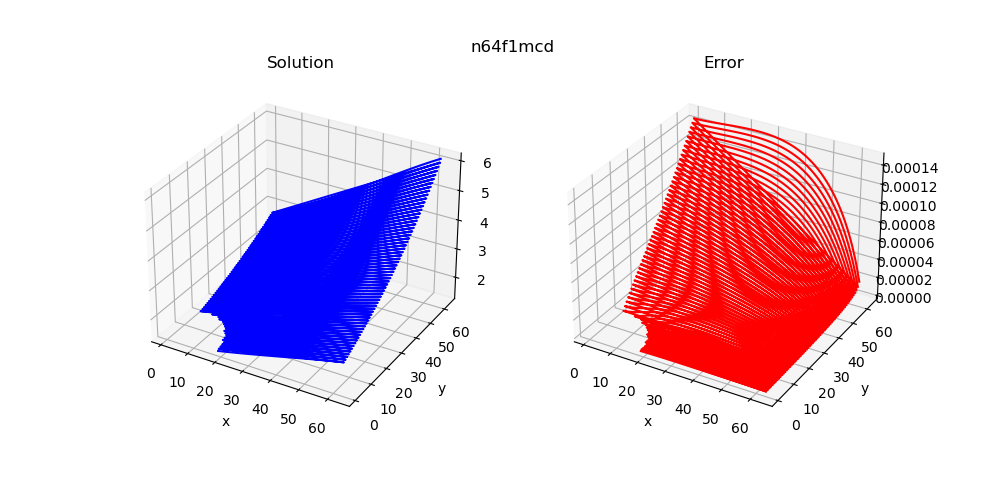
\includegraphics[scale=0.6]{../../image/n64f1mcd.png}
\subsection*{n64f1mcm}
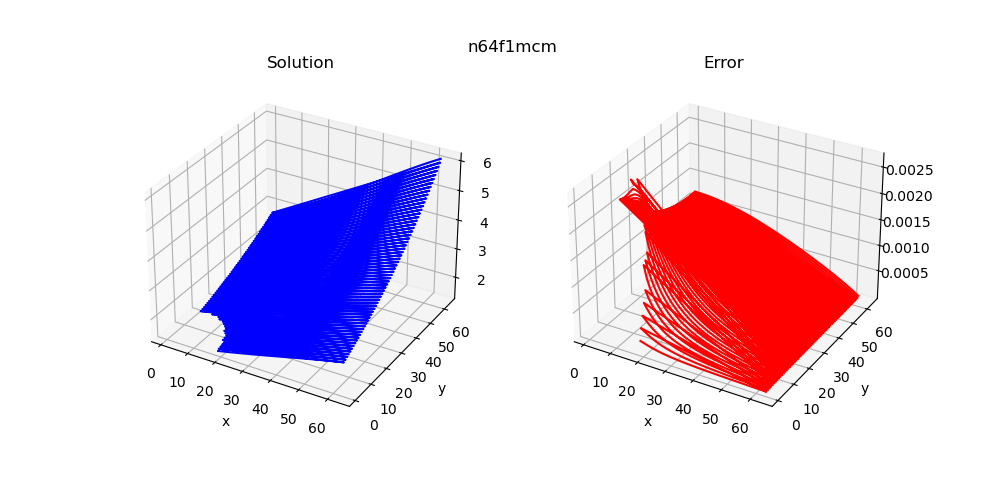
\includegraphics[scale=0.6]{../../image/n64f1mcm.png}

